%%%%%%%%%%%%%%%%%%%%%%%%%%%%%%%%%%%%%%%%%%%%%%%%%%%%%%%%%%%%%%%%%%%%%%%%%%%%
%% Trim Size: 9.75in x 6.5in
%% Text Area: 8in (include Runningheads) x 5in
%% ws-ijait.tex   :   01-10-2014
%% Tex file to use with ws-ijait.cls written in Latex2E.
%% The content, structure, format and layout of this style file is the
%% property of World Scientific Publishing Co. Pte. Ltd.
%%%%%%%%%%%%%%%%%%%%%%%%%%%%%%%%%%%%%%%%%%%%%%%%%%%%%%%%%%%%%%%%%%%%%%%%%%%%
%%

\documentclass{ws-ijait}

\usepackage{epstopdf}
\usepackage{color}
\usepackage{xspace}
\usepackage{booktabs}
\usepackage{placeins}

\usepackage[vlined,ruled,norelsize]{algorithm2e}
\usepackage{amsmath,amssymb,mathtools}

\begin{document}

\newcommand{\red}[1]{{\color{red} #1}}

\markboth{Tom\'a\v{s} K\v{r}en, Martin Pil\'at, Roman Neruda}
{Strongly Typed Genetic Programming for Automatic Creation of Machine-Learning
Workflows}

%%%%%%%%%%%%%%%%%%%%% Publisher's Area please ignore %%%%%%%%%%%%%%%
%
\catchline{}{}{}{}{}
%
%%%%%%%%%%%%%%%%%%%%%%%%%%%%%%%%%%%%%%%%%%%%%%%%%%%%%%%%%%%%%%%%%%%%

\title{Automatic Creation of Machine-Learning Workflows with Strongly Typed
Genetic Programming}


\author{Tom\'a\v{s} K\v{r}en}

\address{Charles University, Faculty of Mathematics and Physics, Malostransk\'e
n\'am\v{e}st\'i 25, 118 00 Prague, Czech Republic, Tomas.Kren@mff.cuni.cz}

\author{Martin Pil\'at}
\address{Charles University, Faculty of Mathematics and Physics, Malostransk\'e
n\'am\v{e}st\'i 25, 118 00 Prague, Czech Republic, Martin.Pilat@mff.cuni.cz}


\author{Roman Neruda}
\address{Institute of Computer Science, The Czech Academy of Sciences, 
Pod Vod\'arenskou v\v{e}\v{z}\'i 271/2, 182 07 Prague, Czech Republic, 
roman@cs.cas.cz}

\newcommand{\ar}{\rightarrow}
\newcommand{\Dlong}{unlabeled data\xspace}
\newcommand{\LDlong}{labeled data\xspace}
\newcommand{\Dshort}{\textit{$D$}\xspace}
\newcommand{\LDshort}{\textit{$LD$}\xspace}
\newcommand{\dia}{\textit{$ens_1$}\xspace}
\newcommand{\diaZero}{\textit{$ens_0$}\xspace}
\newcommand{\splitComb}{\textit{$split$}\xspace}
\newcommand{\cons}{\textit{$cons$}\xspace}

\newcommand{\komb}[1]{\textit{#1}}
\newcommand{\kons}[1]{\textit{#1}}

\newcommand{\Dag}{\kons{Dag}}
\newcommand{\D}{\kons{D}}
\newcommand{\LD}{\kons{LD}}
\newcommand{\Boo}{\kons{Boo}}
\newcommand{\V}{\kons{V}}
\newcommand{\Succ}{\kons{S}}
\newcommand{\Zero}{\kons{0}}
\newcommand{\Same}{\kons{Same}}
\newcommand{\Disjoint}{\kons{Disjoint}}

\newcommand{\Suc}[1]{(\Succ\ #1)}
\newcommand{\Ve}[3]{(\V\ #1\ #2\ #3)}

\newcommand{\DAG}[2]{(\Dag\ #1\ #2)}
\newcommand{\splitter}[4]{\DAG{#1}{\Ve{#2}{#3}{#4}}}
\newcommand{\merger}[4]{\DAG{\Ve{#1}{#3}{#4}}{#2}}
\newcommand{\dvaPlus}[1]{\Suc{\Suc{#1}}}
\newcommand{\dva}{\dvaPlus{\Zero}}


\newcommand{\la}{\leftarrow\xspace}
\newcommand{\op}{\operatorname}
\newcommand{\mgu}[1]{\op{MGU}(#1)}


\newcommand{\Pseudokod}[4]{
	\begin{figure}[!t]
	\removelatexerror
	\begin{algorithm}[H]
		\caption{\label{#4}#1}
		\DontPrintSemicolon
		\SetKwProg{Fn}{function}{}{}
		\Fn{#2}{#3}
	\end{algorithm}
	\end{figure}
}

\makeatletter
\newcommand{\removelatexerror}{\let\@latex@error\@gobble}
\makeatother



\maketitle

\begin{history}
\received{(Day Month Year)}
\revised{(Day Month Year)}
\accepted{(Day Month Year)}
%\comby{(xxxxxxxxxx)}
\end{history}

\begin{abstract}
\end{abstract}

\keywords{Genetic programming; machine learning workflows; asynchronous
evolutionary algorithm}

\section{Introduction}	

In the world of machine learning, ensemble methods -- combinations of more
simple methods -- can improve the quality of models significantly. For example,
in the famous Netflix prize\footnote{http://www.netflixprize.com/}, the winning
model was an ensemble of many simple models which together form a much more
complex and better performing model. Similarly, in most of the
Kaggle\footnote{https://www.kaggle.com/} competition, the winning submission is
an ensemble of potentially tens of different methods. 

Most often, the ensembles are created manually, which is a tedious task that
requires a machine learning expert. One of the difficulties in the task comes
from the fact that there are many machine learning methods and each of them has
its own strengths and weaknesses. This means that for every dataset, one needs
to select a different set of machine learning methods and combine them in a
different way. Moreover, each of the methods can have a number of parameters
which can significantly affect its performance on any given dataset and must
therefore be tuned. For single methods, the tuning can be performed by rather
simple search methods and very often grid search or random search are used.
However, in the ensemble the number of parameters of all the methods grows
linearly with the number of methods and therefore the number of their
combinations which must be tried grows exponentially. 

In this work we deal with automated design of machine learning workflows. A
workflow is a combination of machine learning methods like data preprocessors
and classifiers with other ``helper'' methods that implement different types of
ensembles. In order to create design the workflows and tune their parameters at
the same time, we use typed genetic programming. The type system restricts the
workflows in such a way that they make sense from the machine learning view and
it is possible to evaluate them. For example, it ensures that preprocessing is
applied before classification and not after, or that there is always at least
one classifier in the workflow. At the same time with the design of the
workflow, the genetic programming also performs parameter tuning. To this end,
there is a genetic operator that changes the parameters of the methods in the
workflow.

The method described in this paper (called GP-ML v3) is an extension of methods
we described earlier\cite{SSCI2015,7814654}. The main difference between the
presented version and the previous versions is that now we use a larger number
of base classifiers in the ensembles and also use a better technique for the
generation of typed individuals in the genetic programming. The details of the
two earlier versions will be discussed in the following section.

\section{Related Work}

One of the first problems that need to be solved while creating machine learning
workflows automatically, is to ensure that the workflows make sense. To this end
Panov \emph{et al.}\cite{4734003} and Diamantini \emph{et al.}\cite{Diamant}
used ontologies. 

Others limit the complexity of the workflow in such a way that creating a valid
workflow is easy. Most commonly, the workflow is in fact a pipeline that
contains some preprocessing methods followed by a single classifier or
regressor. Such an approach was used e.g. by Kaz\'ik \emph{et
al.}\cite{aKazikADMI14}. Feurer \emph{et al.}\cite{NIPS2015_5872} were able to
win one phase of the ChaLearn AutoML challenge\cite{7280767} with their method
called auto-sklearn, that uses Bayesian optimization to optimize pipelines with 
one feature preprocessor, three data preprocessors and a single classifier.

Others used a complementary approach of combining results from pipelines of
fixed size. This method was used by Folino and Pisani\cite{MoraaSquirel} who
combined the outputs by genetic programming.

The work presented in this paper is most closely related to the T-POT algorithm 
by Olson \emph{et al.}\cite{Olson2016EvoBIO}. The algorithm also uses genetic
programming to create complex machine learning workflows that can contain a 
number of different machine learning methods and preprocessors. The workflows
resemble a tree, where the data flow from the leaves to the root. Every time
data should be merged, the predictions created by the models before the merging
node are added as features to the set. Following machine learning methods can 
used these predictions in order to create better models.

We have already presented two versions of the GP-ML algorithm. The first
version\cite{SSCI2015} (GP-ML v1) supported only four different classifiers and
a single type of ensemble -- voting. We used a strongly typed genetic
programming with the traditional generational evolutionary algorithm. The
generational algorithm has a serious drawback. It needs to wait for the whole
generation to finish evaluating before it can start working on the next
generation. However, in the design of machine learning workflows, each
evaluation can take a different amount of time. If the algorithm is executed in
a parallel environment (which it should as the evaluation of workflows takes a
lot of time), many of the CPUs are idle while the slowest workflows are
evaluated. This can be slightly improved by using less CPUs than is the
population size, however a much better way is to use asynchronous evolution. In
asynchronous evolution, new individuals are created and submitted for evaluation
as soon as an individual is evaluated. In this way, all the CPUs can be used
effectively during the whole run of the algorithm. The use of asynchronous
evolution and addition of two other ensemble methods -- boosting and stacking is
the main difference between the first version of GP-ML and its second
version\cite{7814654} (GP-ML v2). Asynchronous evolutionary algorithms are known
to be biased towards the faster evaluating parts of the search
space\cite{Scott:2016:EBQ:2908812.2908934}, although in general this may be a
problem, in this case, we consider it an advantage as faster workflows are
preferable to slower ones.

In this paper, we present the newest version of GP-ML (GP-ML v3). The main
difference between this version and the previous version is the addition of six
basic classifiers and, more importantly, a different algorithm for the
generation of individuals in the genetic programming. While the new generating
algorithm should not have a significant direct impact on the quality of
workflows found by GP-ML, it allows the algorithm to work with much larger
individuals, which directly translates to more complicated workflows.



\section{Our approach}

\subsection{Individual representation}

Let us start with brief clarification of what we mean by term machine learning workflow. We can distinguish two kinds of machine learning methods: basic and combined. The basic methods are particular \textit{named} methods such as specific classification, regression, clustering, preprocessing or voting algorithms. On the other hand, the combined methods are \textit{anonymous} results of combining several basic methods into one compound by means of some specific ensemble method (such as stacking or boosting) or by simply putting outputs of one method as inputs to other ones. We call these combined method \textit{machine learning workflows}.

ML workflows are naturally representable as directed graphs; vertices represent basic methods and edges represent flows of data.
Fig. \ref{everything_example}. shows an example of such a workflow containing all above mentioned kinds of basic methods and ensembles.

\begin{figure}[th]
\centerline{\includegraphics[width=13cm]{everything_example.png}}
\vspace*{8pt}
\caption{Example workflow illustrating our range of methods.}
\label{everything_example}
\end{figure}

Each edge has a type corresponding to the type of data flowing through it. 
From the high level machine learning point of view we distinguish two basic types o data;
input \Dlong ($\D$) and output \LDlong ($\LD$) containing the predictions.

Workflow graphs are slightly different from standard graphs in that some of the edges may start nowhere (input edges) or end nowhere (output edges). 
Alternatively we may add two special nodes, \textit{input} and \textit{output}, and let these special edges star or end in them.
One way or another, the special edges determine a \textit{type} of a workflow.

A workflow (such as the one on fig. \ref{everything_example}.) representing a classifier has one input edge of type $\D$ and one output edge of type $\LD$.

To train and evaluate a significant number of such workflows - which may possibly be rather huge beasts -  presents a seriously time consuming task (thanks especially to nested cross-validations). Therefore we decided to take into account only workflows without cycles in their graph, i.e. directed acyclic graphs (DAGs). Doing so we limit the training and evaluation time by limiting the size of generated workflows, since the evaluation time of a DAG workflow is reasonably proportional to the number of basic methods.

Consider a DAG with one input edge of type $a$ and with one output edge of type $b$, then we say that the dag has type $\DAG{a}{b}$. 
For example the DAG from fig. \ref{everything_example} has type $\DAG{\D}{\LD}$ which is the type of a classifier.
Type $\Dag$ is an example of a \textit{parametric type}, that is a type that takes two other types (e.g. $\D$ and $\LD$) as parameters to construct a specific type (e.g. $\DAG{\D}{\LD}$).
Parametric types are extensively used and exploited in our approach.
To deal with DAGs with multiple input or output edges is a slightly more complicated business explained below.

%\subsubsection{DAG combinators}

During the evolution we need to generate and manipulate the workflow individuals. Rather than direct manipulation of the DAGs we prefer an indirect tree representation. From the evolution point of view the individuals are program expressions that may be  evaluated to give a value. This value is a JSON representation of the DAG encoding a ML workflow. This JSON value serves as a blueprint from which the actual ML workflow is build. Thus the DAG representation is an intermediate representation of a workflow.

Our approach to constructing the workflow DAGs is based on strongly typed pure functional programming style. In the terms of classical genetic programming, one specifies a library from which the syntactic trees of program individuals are build by specifying a set of terminals (leaf node symbols) and a set of functions (interior node symbols). 

Roughly speaking, we may say that our terminal set consists of basic machine learning methods and function set consists of dag combinators; operators that connect two or more smaller DAGs in a single more complicated one by some kind of serial or parallel composition. A careful reader may spot that some higher-orderism is in order here, since basic methods are basically functions, thus DAG combinators are functions over functions, i.e. higher-order functions.

We see three major benefits of the tree representation of individuals in comparison with a more direct representation:
\begin{itemlist}
\item Trees are simple yet rich enough structures to support natural ways of substructure manipulation satisfying recombination needs of evolution driven search. Most notably in a cross-over operator.
\item Extensibility. \red{todo napsat ze se to da rozsirovat dalsima symbolama co nerozbijou to stary. Functional programming - simple yet powerful tool for writing extensible programs.}
\item Satisfaction of semantically imposed constraints. Because not all the possible DAGs are meaningful ML workflows. We manage to satisfy these constraints by transforming them onto type level in a way which we are going to demonstrate on the following simple example.
\end{itemlist}
%\subsubsection{Generality and Correctness of the combinators}
In the case of classical untyped genetic programming the terminal and function set consists only of the symbols accompanied with information about number of arguments that each function takes. In the typed situation we accompany the symbols with their types. Since the information whether a symbol is a terminal or function (and its arity) is already contained in the types, we can marge the terminal and function set into one library
%\footnote{\red{poznamka o tom ze v typový teorii se tomu řika context or basis a tak to pouzivame aby se propojila souvyslost.}} 
set $\Gamma$. This merge is also natural for applicative tree notation we use, which is described below.  

Let us consider a small yet illustrative workflow depicted on figure \ref{simple_stacking} together with its tree representation, on which we demonstrate some of our combinators and why they have rather complicated types.

\begin{figure}[th]
\centerline{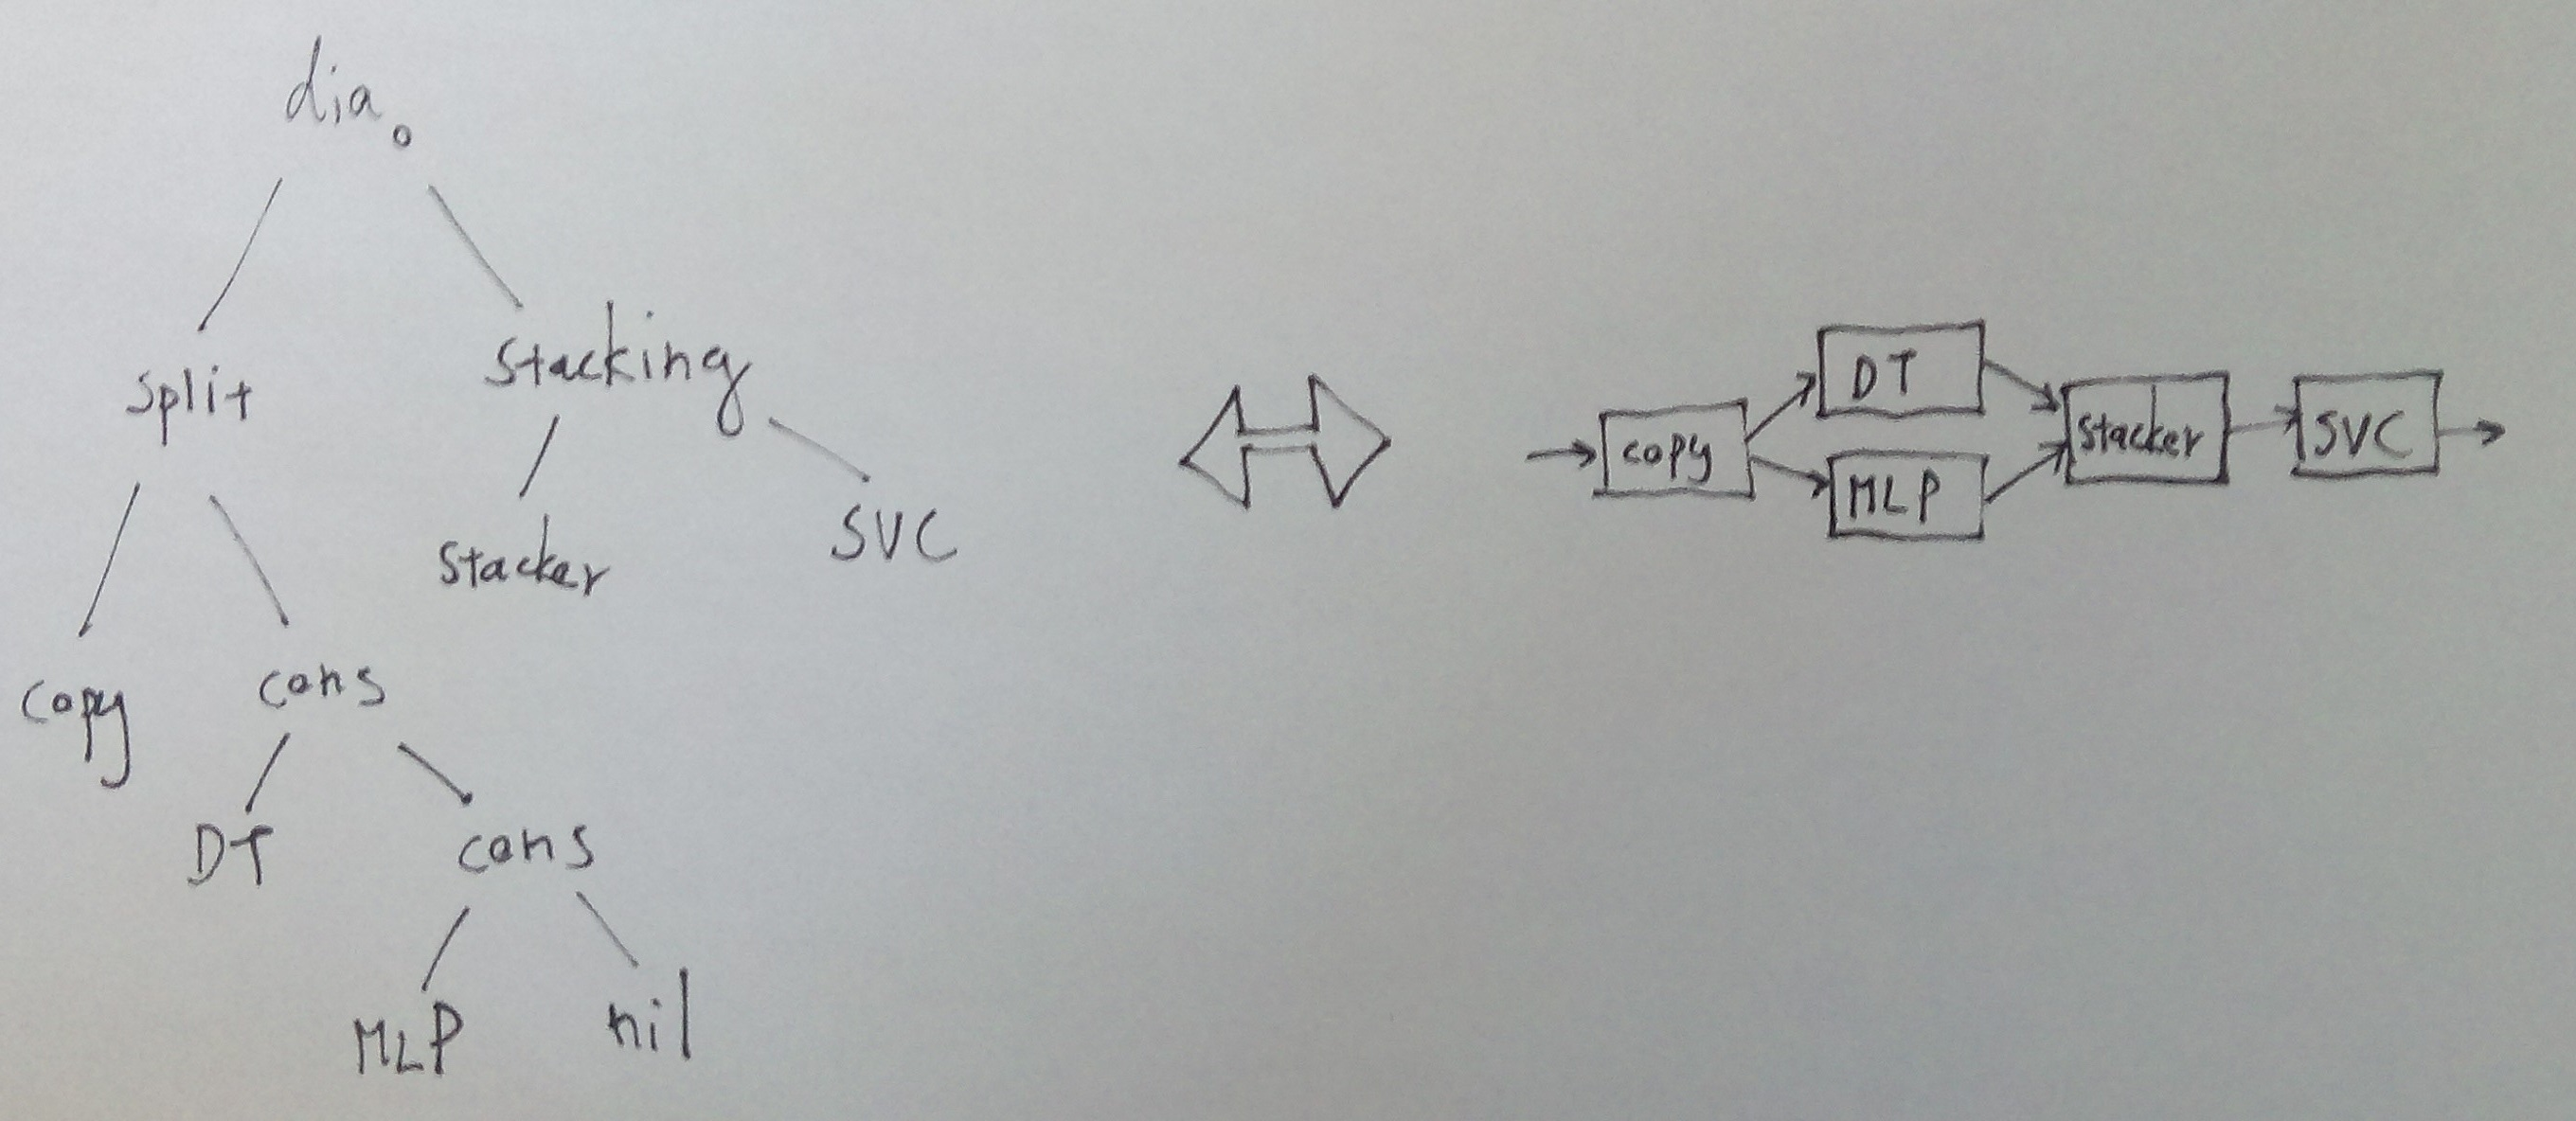
\includegraphics[width=12cm]{simple_stacking.png}}
\vspace*{8pt}
\caption{Simple stacking example.}
\label{simple_stacking}
\end{figure}

Although we internally use more general applicative tree representation (with all the symbols in leaf nodes),
here we present the tree as an S-expression with function symbols in the interior nodes.
Let us start in the root of the tree, where is the $dia_0$ symbol standing for DAG combinator with type:
 
$\splitter{\D}{\LD}{n}{c} \ar \merger{\LD}{\LD}{n}{c} \ar \DAG{\D}{\LD}$
  
So it is a function taking two arguments\footnote{We use the functional convention for functions with multiple arguments discussed below in the subsection about applicative notation.}, 
first of type $\splitter{\D}{\LD}{n}{c}$ and second of type $\merger{\LD}{\LD}{n}{c}$, 
and producing result of type $\DAG{\D}{\LD}$, that is a DAG with one input edge of type $\D$ and one output edge of type $\LD$ representing a classifier model.
We use names starting with uppercase letter for specific (possibly parametric) types (e.g. $\Dag, \D, \LD, \V$) 
and names starting with lowercase letter for \textit{type variables} (e.g. $n, c$).

The result of the $dia_0$ combinator is a combined classifier workflow serially composing its two arguments, which are again workflows but now with a slightly more complicated type in the middle; 
the output type of the first and the input type of the second is the same type $\Ve{\LD}{n}{c}$. 

In general $\Ve{a}{n}{c}$ is type representing a vector of $n$ values of type $a$ 
with a \textit{splitting case} $c$.
In order to explain what a \textit{splitting case} is let us have a look on the DAG of the example workflow on fig. \ref{simple_stacking}. First the input data are copied into two different classification methods and their results are prepared by stacker to by given to the SVC classifier as input data to give the final results. But if we replace the copy splitter with k-means splitter (namely 2-means since the copy to be replaced has two outputs), then the resulting workflow does not make sense any more, because models to be stacked need to be given the same data. The difference between copy and k-means is that although they have the same topology they have different approach to splitting; a copy just makes several \textit{same} copies of the input data, whereas k-means (or any clustering method in general) splits the input data into several \textit{disjoint} sub-parts. We call this splitting approach a \textit{splitting case} and distinguish two types of cases: $\Same$ and $\Disjoint$. Another thing worth mentioning is that we manage a size of a vector on the type level via the type parameter $n$.

From $dia_0 : \splitter{\D}{\LD}{n}{c} \ar \merger{\LD}{\LD}{n}{c} \ar \DAG{\D}{\LD}$ we see that
the number $n$ of output edges of the first DAG may be arbitrary but it must match the number of input edges of the second, similarly for the splitting case $c$ resulting in that stacker merger is preceded by suitable splitter. The type of $dia_0$ contains type variables which means that $dia_0$ is a \textit{polymorphic} function, i.e. it can match many specific types matching the general pattern. 
As we will go through the rest of the example we will see that the actual types of the subtrees are  instances of the types of the parameters of the $dia_0$ combinator. Let us move to the left son.

$split : \splitter{\D}{\D}{n}{c} \ar \Ve{\DAG{\D}{\LD}}{n}{c} \ar \splitter{\D}{\LD}{n}{c}$

We see that this combinator again takes two inputs; 
the first is a DAG with one input edge of type $\D$ and with $n$ output edges of type $\D$,
the second is a vector of $n$ classifiers
and the result is a DAG with one input edge of type $\D$ and with $n$ output edges of type $\LD$ 
(thus perfectly matching the type of the first input of $dia_0$).
From the type alone one may guess what this combinator does; it serially connects the first dag
with a DAG resulting from parallel composition of all the classifiers in the vector given as second input.

Now we get to the first leaf $copy$, which has type $\splitter{\D}{\D}{\dvaPlus{n}}{\Same}$. We encode the numbers on the type level in the standard unary way. The type of $copy$ matches the type of the first argument of $split$, but now it is a more specific instance specifying the \textit{splitting case} to $\Same$ and by $\dvaPlus{n}$ it guarantees that the number of its output edges is at least 2.      

At this point we discontinue the detailed examination of the example. \textbf{Table \ref{tab:gamma}} lists the complete list of our ML workflow library $\Gamma$.

\begin{table}[ht]
\tbl{Our ML workflow library $\Gamma$, all the tree symbols with their types. \label{tab:gamma}}
{\begin{tabular}{ll}
\toprule
symbol 				& type      \\
\toprule
dia$_0$ & $\splitter{\D}{\LD}{n}{c} \ar \merger{\LD}{\LD}{n}{c} \ar \DAG{\D}{\LD}$ \\
dia$_1$ & $\DAG{\D}{\D} \ar \splitter{\D}{\LD}{n}{c} \ar \merger{\LD}{\LD}{n}{c} \ar \DAG{\D}{\LD}$ \\
split   & $\splitter{\D}{\D}{n}{c} \ar \Ve{\DAG{\D}{\LD}}{n}{c} \ar \splitter{\D}{\LD}{n}{c}$ \\
cons    & $a \ar \Ve{a}{n}{c} \ar \Ve{a}{\Suc{n}}{c}$ \\
nil     & $\Ve{a}{\Zero}{c}$ \\
\colrule
PCA     & $\DAG{\D}{\D}$ \\
kBest   & $\DAG{\D}{\D}$ \\
\colrule
kMeans  & $\splitter{\D}{\D}{\dvaPlus{n}}{\Disjoint}$ \\
copy    & $\splitter{\D}{\D}{\dvaPlus{n}}{\Same}$ \\
\colrule
SVC        & $\DAG{\D}{\LD}$ \\
logR       & $\DAG{\D}{\LD}$ \\
gaussianNB & $\DAG{\D}{\LD}$ \\
DT         & $\DAG{\D}{\LD}$ \\
Perceptron & $\DAG{\D}{\LD}$ \\
SDG        & $\DAG{\D}{\LD}$ \\
PAC        & $\DAG{\D}{\LD}$ \\
LDA        & $\DAG{\D}{\LD}$ \\
QDA        & $\DAG{\D}{\LD}$ \\
MLP        & $\DAG{\D}{\LD}$ \\
\colrule
stacking   & $\merger{\LD}{\D}{n}{\Same} \ar \DAG{\D}{\LD} \ar \merger{\LD}{\LD}{n}{\Same}$ \\
stacker    & $\merger{\LD}{\D}{\dvaPlus{n}}{\Same}$ \\
\colrule
boosting & $\DAG{\D}{\Boo} \ar \Ve{\DAG{\Boo}{\Boo}}{\dvaPlus{n}}{c} \ar \DAG{\Boo}{\LD} \ar \DAG{\D}{\LD}$ \\
booBegin   & $\DAG{\D}{\Boo}$ \\
booster    & $\DAG{\D}{\LD} \ar \DAG{\Boo}{\Boo}$ \\
booEnd     & $\DAG{\Boo}{\LD}$ \\
\botrule
\end{tabular}}
\end{table} 

\red{Rict ze typ tech subtermu jsou takovy a makovy a ze to teda rezultuje v takovou a makovou substituci, aby pak bylo normalni ji pouzit nize}

We may say that our approach balances two mutually counteractive tendencies: generality and correctness. Correctness is ensured by encoding the constraints into the type level, yet the combinators may remain general thanks to parametric polymorphism.




%\subsubsection{Applicative representation of program trees}

The standard way of tree representation of tree individuals in genetic programming uses S-expressions,
i.e. an interior node represents a function with its argument sub-expressions in its direct sub-trees. 
Thus terminal symbols are in leaf nodes and function symbols are interior nodes.
On the other hand, there is a more general \textit{applicative} representation, which has all symbols in leafs and all the interior nodes are of one kind: binary explicit application operator.

This is possible thanks to the fact that all function with multiple inputs may be considered a function with one input. For example function $f : A_1 \times A_2 \ar B$ can be thought of as having type $f^\prime : A_1 \ar (A_2 \ar B)$ abbreviated as $f^\prime : A_1 \ar A_2 \ar B$. Function $f^\prime$ given a first input returns another function which given a second input returns the result of original function $f$. So instead of all at once application $f(x,y)$ we apply arguments sequentially as $f^\prime(x)(y)$. This technique is called \textit{currying}. Applicative tree representation explicitly captures those binary applications.

\begin{figure}[th]
\centerline{\includegraphics[width=12cm]{simple_stacking_app.png}}
\vspace*{8pt}
\caption{Simple stacking example: S-expresion and applicative representation.}
\label{simple_stacking_app}
\end{figure}

The applicative representation is more general then S-expressions because now the function may be represented as an sub-expression, whereas S-expression notation allows only single symbols to act as functions (interior node can hold only a single function symbol, but not a whole expression).

With more general tree representation comes more general crossover. E.g. now the tree-swapping crossover can also swap functions, so from the S-expression point of view it can swap interior nodes, because in applicative representation all the symbols are in leafs.  

\subsection{Generating}

\newcommand{\sigmaPr}{\sigma^\prime}
\newcommand{\tauPr}{\tau^\prime}
\newcommand{\xPr}{x^\prime}
\newcommand{\nPr}{n^\prime}
\newcommand{\nPrr}{n^{\prime\prime}}
\newcommand{\nPrrr}{n^{\prime\prime\prime}}
\newcommand{\tausPr}{\tau_s^\prime}
\newcommand{\s}{\sigma}
\newcommand{\Th}{\theta}
\newcommand{\sPr}{\sigmaPr}
\newcommand{\thPr}{\theta^\prime}



\newcommand{\then}{\Rightarrow}
\newcommand{\E}[2]{(\exists #1)\ #2}
\newcommand{\A}[2]{(\forall #1)\ #2}
\newcommand{\Ain}[3]{(\forall #1 \in #2)\ #3}


\newcommand{\ap}[2]{(#1\,#2)}
\newcommand{\defi}{\coloneqq}
\newcommand{\defe}{\mathrel{\vcentcolon\equiv}}


\newcommand{\inhab}[1]{\op{I}(#1)}

\newcommand{\tord}{\preccurlyeq}
\newcommand{\stord}{\prec}
\newcommand{\ordt}{\tord_\tau}
\newcommand{\tek}{\sim}
\newcommand{\ntek}{\nsim}
\newcommand{\ekt}{\tek_\tau}
\newcommand{\nekt}{\ntek_\tau}
\newcommand{\nsucct}{\nsucc_\tau}

\newcommand{\MGI}[1]{\op{MGI}(#1)}
\newcommand{\MGIt}{\MGI{\tau}}
\newcommand{\It}{\op{I}(\tau)}

\newcommand{\ids}{\sigma_{\op{id}}}

\newcommand{\U}[2]{\op{U}(#1,#2)}
\newcommand{\Utt}{\U{\tau}{\tauPr}}
\newcommand{\MGUtt}{\MGU{\tau}{\tauPr}}

%\newcommand{\e}[2]{\op{E}_{#1}(#2)}
\newcommand{\e}[2]{\op{E}(#1,#2)}
\newcommand{\restrict}[2]{{#1}_{\mid #2}}
\newcommand{\fresh}[2]{\op{fresh}_{#1}(#2)}
\newcommand{\newVar}[1]{\op{newVar}(#1)}
\newcommand{\Ss}[1]{\op{ss}(#1)}
\newcommand{\TS}[2]{\op{ts}_{#1}(#2)}
\newcommand{\ts}[2]{\op{ts}_{#1}(#2)}
\newcommand{\TSij}[3]{\op{ts}_{#1,#2}(#3)}
\newcommand{\trees}[2]{\op{trees}_{#1}(#2)}
\newcommand{\FX}{\ap{F}{X}}
\newcommand{\sF}{\s_{F}}
\newcommand{\sX}{\s_{X}}
\newcommand{\vars}[1]{\op{vars}(#1)}
\newcommand{\dom}[1]{\op{dom}(#1)}
\newcommand{\IH}{induction hypothesis\xspace}
\newcommand{\discup}{~\mathbin{\dot{\cup}}~}

\newcommand{\abs}[1]{\lvert #1 \rvert}



\newcommand{\nv}{v}
\newcommand{\nvPr}{\nv^\prime}


%- Dosud jsme popsali co je cílem tvořit a co to omezuje, aby to dávalo smysl. Ted popíšem jak na to jdeme. Nejprve to ilustrujem jednoduchym prikladem to provide a context, pak formalneji predstavime 

We present the general notions on which our novel tree generating method is based and after that we describe the algorithm together with brief mention of techniques which make it fast enough for massive use in individual generating and in mutation operation.

%Na to neni čas
%\subsubsection{A simple example}
%- to by šlo snad názorně ukázat na příkladě generování stromu k>1:
%- Generujem Dag D LD, k>1 -> v kořeni stromu je aplikace tedy:
%- levej syn je funkce z něčeho do (Dag D LD), pravej syn je to něco
%… az se dostanem do listů (strom velikosti 1) - výběr symbolu z gammy aby to pasovalo..

%\subsubsection{Generating based on sizes}
%- 1. základ našeho přístupu: generuje strom pro danou velikost stromu (počet symbolů).
%  - což mimojiné umožnuje mnohem přímější kontrolu nad tím, z jakého rozložení taháme naše jhedince 
%  - zde popsat to jak to děláme (32, 16,16, 8,8,8,8, ...)


%\subsubsection{Existential queries}

Our approach to generating algorithm is based on queries of a form $(k,\tau)$ where $k$ is the size (number of symbols) of a tree $M$ that we want to generate and $\tau$ is a \textit{goal type}. A \textit{goal type} $\tau$ is not necessary type of $M$, rather it is a type which may be instantiated to a more special type $\tauPr$ such that $M : \tauPr$. A type $\tauPr$ is an instance of type $\tau$ if there is a \textit{substitution} $\s$ such that $\tauPr = \s(\tau)$. 

%\red{todo: Kdyz bude cas tak vysvetlit na priklade  $a \ar b$ ze je nobydlenej ale pro sub $b = a$ je obydlenej identitou.}

We may define the set $\e{k}{\tau}$ of all the trees that fit the query $(k,\tau)$ in the following way.
\begin{align*}
\e{k}{\tau} \defi& \{ M \mid \E{ \op{substitution} \s}{ M : \s(\tau) }, \abs{M} = k \}
\end{align*}
This definition is declarative and hints us nothing about how to actually construct such trees.
Thus our strategy is to make a constructive way of enumerating trees of $\e{k}{\tau}$ 
which is still mathematical so that it can be rigorously shown that it is equivalent to the declarative definition. 
After that we lift those constructive definitions to obtain a generating algorithm well suited for generation of one tree individual of a given size $k$ and respecting a given goal type $\tau$.
Let us briefly outline this whole process.

In order to do so we gradually define set $\ts{k}{\tau,\nv}$ where $k$ and $\tau$ are size and goal type as in the $(k,\tau)$ query and $\nv$ is a rather technical argument needed for maintaining fresh type variables; $\nv$ is a next fresh type variable index that can be safely used when a fresh variable is needed (confused reader may ignore them). An element $(M,\s,\nvPr) \in \ts{k}{\tau,\nv}$ is a tree $M$ together with some useful information; most general $\s$ such that $M : \s(\tau)$ and $\nvPr$ is a new (possibly updated) next variable index. 
Let us start with $k = 1$:
\begin{align*}
\ts{1}{\tau,\nv_0} \defi&  \{ (s,\restrict{\mu}{\tau}, \nv_1) \mid \\
  & ~~ (s : \tau_s) \in \Gamma, \\
  & ~~ (\tausPr,\nv_1) = \fresh{\tau}{\tau_s, \nv_0}, \\
  & ~~ \mu = \mgu{\tau,\tausPr}
\}
\end{align*}
Let us comment on this definition from the algorithmic point of view. In order to know which trees of size 1 match a given goal type $\tau$ we need to iterate though the whole library $\Gamma$. 
For each symbol $s$ with assigned type $\tau_s$ in $\Gamma$ we check whether $\tau_s$ can be matched with the goal type $\tau$ by trying to find the \textit{most general unifier} (MGU), but before we do so we must make $\tausPr$ a fresh copy of $\tau_s$ in order to avoid unwanted  type variable clashes.
Finally we restrict the domain of substitution $\mu$ only to type variables of $\tau$, so that it does not contain irrelevant variables of $\tausPr$.  

For $k > 1$, from point of view of applicative representation, we know that such tree must be an application of the form $\FX$. Let us first consider situation, where we know the sizes of the subtrees $F$ and $X$; let $\abs{F} = i$ and $\abs{X} = j$, then:
\begin{align*}
\ts{i,j}{\tau,\nv_0} \defi& \{ (\FX, \restrict{(\sX \circ \sF)}{\tau}, \nv_3) \mid \\ 
  & ~~ (\alpha, \nv_1) = \newVar{\tau,\nv_0}, \\
  & ~~ (F,\sF,\nv_2) \in \ts{i}{\alpha \ar \tau,\nv_1}, \\
  & ~~ (X,\sX,\nv_3) \in \ts{j}{\sF(\alpha), \nv_2} 
\}
\end{align*}
In order to generate a tree of a form $\FX$ for which its type matches $\tau$, 
we need to generate a function tree $F$ which returns something matchable with $\tau$, and 
we need to generate a argument tree $X$ which matches the input type of generated $F$.
In other words, first we need to generate $F \in \e{i}{\alpha \ar \tau}$, where $\alpha$ is a new
type variable such that it does not clashes with any preexisting type variable.
This can be achieved by taking an element $(F,\s_F,\nv_2) \in \ts{i}{\alpha \ar \tau,\nv_1}$.
Together with tree $F$ we also get a substitution $\s_F$, such that 
$\s_F(\alpha \ar \tau)$ is the most general type matching $\alpha \ar \tau$ 
for which holds $F : \s_F(\alpha \ar \tau)$. 
Now that we fixed tree $F$ we need to generate $X$ matching $\s_F(\alpha)$.
Again, this can be achieved by taking an element $(X,\sF,\nv_3) \in \ts{j}{\s_F(\alpha),\nv_2}$.
Now we have both $F$ and $X$ and may return the $\FX$, together with 
restricted composition of $\sF$ and $\sX$, and with auxiliary $v_3$ for maintaining the fresh type variables sound.

Finally we can define $\ts{k > 1}{\tau,n}$ by the means of $\ts{i,j}{\tau,n}$ 
for each applicable $i$ and $j$ such that $i+j = k$.
\begin{align*}
\ts{k > 1}{\tau,\nv} \defi& \bigcup\limits_{i=1}^{k-1}  \TSij{i}{k-i}{\tau, \nv}
\end{align*}


%\subsubsection{Counting the trees}

The $\op{ts}_k$ algorithm is designed for enumeration of trees, but randomly generating a tree is related but more difficult problem. The basic trick how we transform this enumeration into one random tree generation lies in counting the number of trees for a given query.

The first lifting we do is that we transform the $\op{ts}_k$ algorithm dealing with specific trees and their substitutions into a $\op{subs}_k$ algorithm which focuses more on the substitutions and throws away the actual trees, but it still keeps track of the number of trees for a given substitution.  

For an element of $(n,\s,\nvPr) \in \op{subs}_k(\tau,\nv)$ holds that:
$$n = \abs{\{ M \mid (M,\s, \_) \in \ts{k}{\tau,\nv} \}}$$

In other words, $\op{subs}_k$ is a version of $\op{ts}_k$ concerned more with the substitutions then the actual trees, which packs together trees with the same substitution, but it throws away the actual trees and keeps only their count. The implementation of the $\op{subs}_k$ algorithm is very similar to the $\op{ts}_k$ algorithm, only with one additional step of \textit{"packing"} the substitutions.
However, for the most libraries $\Gamma$ the size of $\op{subs}_k$ is greatly smaller then the size of $\op{ts}_k$ and can be cached for relevant queries up to some reasonable $k$. This caching of previous results of $\op{subs}$ for various queries is the core feature enabling fast tree generating.  

%\subsubsection{Final overview of generating}

\newcommand{\ball}{\op{treeID}}

\Pseudokod{Generate a random tree individual for query $(k,\tau)$.}
{\textbf{randomTree}($k,\tau$)}{
	\textbf{random} $\ball \in \{0,\dots,\op{getNum}(k,\tau)-1\}$ \;
	\Return $\op{getTree}_k(\tau,\ball, 0)$
}{randomTree}

\Pseudokod{Get tree individual of size 1.}
{\textbf{getTree$_1$}($\tau$, $\ball$, $\nv_0$)}{
	\For {$(s : \tau_s) \in \Gamma$}{
		$(\tau_s^{\prime},\nv_1) \la fresh_\tau(\tau_s,\nv_0)$ \;
		\If {$\exists ~ \mu = \mgu{\tau,\tau_s^{\prime}}$} {
			\If {$\ball = 0$} {
				\Return $(s:\mu(\tau), \nv_1)$
			} \Else {
				$\ball \la \ball - 1$				
			}
		}	
	}
}{genOne1}

\Pseudokod{Get tree individual of size $k > 1$.}
{\textbf{getTree$_{k>1}$}($\tau$, $\ball$, $\nv_0$)}{
	\For {$i \in \{1,\dots,k-1\}$}{
		$j \la k - i$ \;
		$(\alpha, \nv_1) \la newVar(\tau,\nv_0)$ \;
		\For {$(n_F,\sigma_F,\nv_2) \in subs_i(\alpha \ar \tau, \nv_1 )$}{
			\For {$(n_X,\sigma_X,\nv_3) \in subs_j(\sigma_F(\alpha), \nv_2 )$}{
				$n_{FX} \la n_F \cdot n_X $ \;
				\If {$\ball < n_{FX}$} {
					\textbf{random} $\ball_F \in \{0,\dots,n_F - 1\}$ \;
					\textbf{random} $\ball_X \in \{0,\dots,n_X - 1\}$ \;					
					$(F, \nv_4)  \la getTree_i(\overline{\sigma_F(\alpha \ar \tau)}, \ball_F,\nv_3)$ \;
					$(X, \nv_5) \la getTree_j(\overline{\sigma_X(\sigma_F(\alpha)}), \ball_X,\nv_4)$ \;
					\Return $((F~X) : \sigma_X(\sigma_F(\tau)), \nv_5)$				
				} \Else {
					$\ball \la \ball - n_{FX}$				
				}			
			}
		}	
	}
}{genOneK}

\textbf{Algorithm \ref{randomTree}} shows how a random tree for query $(k, \tau)$ is generated. The number\footnote{The tree counts are huge, thus arbitrary precision integers are required.} of trees for $(k,\tau)$ is computed as follows.

$$\op{getNum}(k,\tau) \defi \smashoperator[r]{\sum_{(n,\_,\_) \in \op{subs}_k(\tau,0)}}n$$

A random $\ball$ is picked from the range given by this count. 
Then the procedure \textit{getTree}, the simplified core of the algorithm, is called. 
The \textit{getTree} is split to two cases based on $k$. 
In a way, we may see \textbf{Algorithm \ref{genOne1}} and \textbf{Algorithm \ref{genOneK}} as 
second liftings of the $\op{ts}_1$ and $\op{ts}_{k > 1}$ algorithms.

The most notable part is when the recursive calls are made in \textbf{Algorithm \ref{genOneK}}.
The condition $\ball < n_{FX}$ indicates that we are in the correct combination of for iterations
corresponding to the given $\ball$. We know the specific instances of sub-tree types, but we need to 
fixate them, because "$\tau$" input of the \textit{getTree$_k$} procedure is interpreted as something that may be instantiated, but we want to stop these instantiations from happening, since we have arrived at the desired type. 
This can be achieved by a trick denoted as overline over the types; 
operation $\overline{\tau}$ denotes replacement of all the type variables of $\tau$ by special \textit{type symbols} never used in any type of $\Gamma$. In a way, this operation is related to the skolemization in logic.

% Our generating algorithm's ambition is to generate the trees uniformly. \red{ "semi-unfiromní" generování - pozn o nedokonalosti }

The presented algorithms are simplified versions of the actual algorithm, which need to deal with caching and caching related technical issues. Another point worth mentioning is that type normalization is done before a query result is queried (and denormalization after the result is returned), since many types are isomorphic to some other types. The normalization used in the implementation results in that types same up to renaming of type variables are considered same and cached only once.



\section{Experiments}

In this section, we describe the experiments we performed in order to evaluate
the quality of GP-ML. The algorithm is compared to a baseline, which consists of
the performance of all the methods used in the ensembles with tuned parameters.
We also compare the current version of GP-ML to its two previous
versions\cite{SSCI2015,7814654}.

\subsection{Datasets}

We performed extensive testing of the GP-ML algorithm on four datasets from the
UCI machine learning repository\cite{Lichman:2013}. These are 
winequality-white\cite{Cortez2009547} (referred to as `wine' in the rest of the paper),
wilt\cite{Johnson:2013:HPA:2512892.2512894}, magic\cite{Bock2004511},  and ml-
prove\cite{Bridge}. The datasets come from different areas and have  different
interesting features. In the wine dataset, the goal is to predict  the quality
of white wine on a scale 1-9 based on its chemical and physical  properties. The
wilt dataset aims to classify images into two classes based on features from
different image analysis approaches. The magic dataset contains  data from the
field of particle physics -- the goal is to predict whether an observation is a
gamma particle or not. Finally, the ml-prove dataset contains information on
different tasks from automated theorem proving. The goal is to  predict which
automated provers would perform the best for each task. The wine and wilt
datasets both contain about 5,000 instances. The wine dataset has 11 attributes
and the wilt dataset has 6 attributes. The other two datasets are larger -- 
ml-prove has over 6,000 instances with 51 attributes and magic has more than 
19,000 instances with 10 attributes.

\subsection{Workflow Components}

\begin{table}[p]
\tbl{The possible values of hyper-parameters for the machine learning methods.
$N$ is the number of attributes in the dataset.
\label{tab:hyperparameters}}
{\begin{tabular}{ll}
\hline
\multicolumn{2}{c}{Support Vector Classifier} \\
\hline
C & \{0.1, 0.5, 1, 2, 5, 10, 15\} \\
gamma & \{0.0, 0.0001, 0.001, 0.01, 0.1, 0.5\} \\
tol & \{0.0001, 0.001, 0.01\} \\
\hline
\multicolumn{2}{c}{Logistic Regression (penalty=l2, solver=sag)} \\
\hline
C & \{0.1, 0.5, 1, 2, 5, 10, 15\} \\
tol & \{0.0001, 0.001, 0.01\} \\
\hline
\multicolumn{2}{c}{Decision Tree Classifier} \\
\hline
criterion & \{gini, entropy\} \\
max\_features & \{0.05, 0.1, 0.25, 0.5, 0.75, 1\} \\
max\_depth & \{1, 2, 5, 10, 15, 25, 50, 100\} \\
min\_samples\_split & \{1, 2, 5, 10, 20\} \\
min\_samples\_leaf & \{1, 2, 5, 10, 20\} \\
\hline
\multicolumn{2}{c}{Perceptron} \\
\hline
penalty & \{'None', 'l2', 'l1', 'elasticnet'\} \\
n\_iter  & \{1, 2, 5, 10, 100\} \\
alpha & \{0.0001, 0.001, 0.01\} \\
\hline
\multicolumn{2}{c}{SGD} \\
\hline
penalty & \{'none', 'l2', 'l1', 'elasticnet'\} \\
loss & \{'hinge', 'log', 'modified\_huber', 'squared\_hinge', 'perceptron'\} \\
n\_iter & \{5, 10, 100\} \\
alpha & \{0.0001, 0.001, 0.01\} \\
l1\_ratio & \{0, 0.15, 0.5, 1\} \\
epsilon & \{0.01, 0.05, 0.1, 0.5\} \\
learning\_rate & \{'constant', 'optimal'\} \\
eta0 & \{0.01, 0.1, 0.5\} \\
power\_t & \{0.1, 0.5, 1, 2\} \\
\hline
\multicolumn{2}{c}{PAC} \\
\hline
loss & \{'hinge', 'squared\_hinge'\} \\
C & \{0.1, 0.5, 1.0, 2, 5, 10, 15\} \\
\hline
\multicolumn{2}{c}{LDA} \\
\hline
solver & \{'lsqr', 'eigen'\} \\
shrinkage & \{None, 'auto', 0.1, 0.5, 1.0\} \\
\hline
\multicolumn{2}{c}{QDA} \\
\hline
reg\_param & \{0.0, 0.1, 0.5, 1\} \\
tol & \{0.0001, 0.001, 0.01\} \\
\hline
\multicolumn{2}{c}{MLP} \\
\hline
activation & \{'identity', 'logistic', 'relu'\} \\
solver & \{'lbfgs', 'sgd', 'adam'\} \\
alpha & \{0.0001, 0.001, 0.01\} \\
learning\_rate & \{'constant', 'invscaling', 'adaptive'\} \\
tol & \{0.0001, 0.001, 0.01\} \\
max\_iter & \{10, 100, 200\} \\
learning\_rate\_init & \{0.0001, 0.001, 0.01\} \\
power\_t & \{0.1, 0.5, 1, 2\} \\
momentum & \{0.1, 0.5, 0.9\} \\
hidden\_layer\_sizes & \{(100,), (50,), (20,), (10,)\} \\ 
\hline
\multicolumn{2}{c}{PCA} \\
\hline
whiten & \{true, false\} \\     
n\_components & \{$\lfloor k \cdot N \rfloor | k \in$ \{0.01, 0.05, 0.1, 0.25, 0.5, 0.75, 1\} \\
\hline
\multicolumn{2}{c}{kBest} \\
\hline
k & \{$\lfloor k \cdot N \rfloor | k \in$ \{0.01, 0.05, 0.1, 0.25, 0.5, 0.75, 1\} \\
\hline
\end{tabular}}
\end{table} 

All the machine learning workflows consists of different types of components,
these are data splitters, data mergers, pre-processors, classifiers and
ensembles. 

The data splitter take a dataset and split it into multiple parts. These parts
are then processed independently by different parts of the workflow. GP-ML
currently uses two types of splitters. The simpler of them is the copy splitter.
It simply takes the dataset and copies it multiple times. The copies are then
processed independently. The other splitter is based on the $k$-means clustering
algorithm. It finds $k$ clusters in the data and each of the clusters is again 
processed independently by other parts of the workflow.

Each splitter must be later in the workflow followed by a merger. The mergers
take multiple predictions made by preceding parts of the workflow and combine
them together to obtain a single prediction. There are two types of mergers --
vote and union. The vote merger computes the number of times each class is
predicted for each instance and outputs the most common prediction as the only
one for that instances. The union merger is used in conjunction with $k$-means
splitter, it combines the results from the different parts of workflows in order
to assign a class to all the instances. In fact, both these mergers are
implemented as the voting marger. Each instances has an unique id, which is
propagated through the system. Once the voting merger gets the results from all 
the methods preceding it, it computes the most common class assignment for each
of these and returns it. In case the data were split by the $k$-means splitter
there is exactly one class assignment for each instance, which is therefore the 
most common.

We use two types of preprocessing methods - the principal component analysis,
and $k$-best which selects $k$ attributes most correlated to the target class.

The set of classifier is different between the two older versions of GP-ML and
the current version. The two oldest versions of GP-ML used support vector
classification (SVC), logistic regression (LR), gaussian naive Bayes classifier
(GNB), and decision trees (DT) as the classifiers. In the current version of
GP-ML we also added perceptron (Perc), linear discriminant analysis (LDA),
quadratic discriminant analysis (QDA), passive aggressive classifier (PAC), SGD
classifier (SGD), and multi-layered perceptron (MLP) to the set of available
base classifiers. 

In the first version of GP-ML, voting was the only type of ensemble supported.
It is implemented in the form of the voting merger and simply counts the number
of times different machine learning methods predict a class for an instance and
chooses the most common class as the resulting one. In the second version of
GP-ML, we added support for two additional types of ensembles - stacking and
boosting.

The stacking ensemble takes another sub-workflows as parameters, computes their
output and creates a new dataset from the outputs of the sub-workflows. Each of
the outputs is a single attribute in the new dataset and the target is the same
as the one for the internal workflows. The resulting new dataset can be used
further in the workflow to produce better models that use the outputs of the
sub-workflows as their inputs. In a sense, the stacking is a generalized version
of the voting, where instead of taking the most common prediction, a model is
trained to combine the prediction of the sub-models. In order to obtain unbiased
prediction from the sub-workflows (i.e. the sub-workflows do not predict the
data they were trained on), we in fact run a five fold cross-validation in
stacker. The input to the stacker is divided into five parts, each time the 
internal models are trained on four of the parts and predict the fifth part. The
prediction from the five folds are combined to obtain the resulting prediction.
This also means that if there is a stacking inside one of the sub-workflows, the
training can take a lot of time.

The boosting ensemble implements the AdaBoost algorithm\cite{FREUND1997119}. The
basic idea is to repeat the learning iteratively, with different weights for
instances in each iteration. Instances which were predicted incorrectly get
larger weight, so that the next classifier puts more emphasis on them. In GP-ML
the boosting is more general -- instead of using the same type of classifier, we
again use another sub-workflows. Each of these sub-workflows may also be
different from the others used in the boosting. One of the assumption of
boosting is that the classifiers support weighted samples. This is unfortunately
not true for all of the classifiers we use in this work. Therefore, in case a
classifier that does not support sample weights is used inside boosting, the
weights are ignored. A better alternative would be to ensure that only
classifiers that support sample weights are used in boosting, however the type
system we use now does not support this.

Many of the machine learning methods mentioned in the previous paragraph have a
number of hyper-parameters which need to be set correctly in order to achieve
the optimal performance. For each of these parameters, we selected a range of
suitable values and the genetic programming evolved the values of the parameters
together with the whole workflow (only values from the specified set can be used
by the GP). All the possible values of the parameters for those methods that
have any parameters are presented in Table~\ref{tab:hyperparameters}. We used
the implementation from the scikit-learn library and all parameters not
mentioned here use their default values.

While the typed genetic programming can ensure that all the workflows are valid
from the machine learning point of view, there may be some situations where the
training of a model in the workflow fails. The most common reasons for failure
are caused by the data itself and cannot be completely avoided -- for example,
if the dataset is split multiple times using the $k$-means splitter, in some
parts of the workflow the number of instances may be too low to fit a model.
Many of the models also fail to operate in cases where there is only one class
for all the instances on their input, however we solved this problem by checking
for this situation and replacing the model that cannot be trained by a constant
model which always outputs the single class. In case an evaluation fails, the
workflow is assigned zero fitness and is immediately removed from the
population.

\subsection{Evaluation Metric}

We used the quadratic weighted $\kappa$ as the metric for the evaluation in all
the datasets except magic. The quadratic weighted $\kappa$ expresses how well a
classifier agrees with the ground truth. It is especially suited for grading
tasks (wine) or binary classification tasks where one of the classes are much
less common than the other one. The values of $\kappa$ are always between -1 and
1, where 1 means complete agreement between the classifier and the ground truth,
-1 means  compete disagreement and 0 is as  good as random guessing. For the
magic dataset, we used the accuracy as the metric optimized by GP-ML, because
the problem has five classes which have no ordering and thus, the $\kappa$
values would make no sense. All values presented in this paper are results of
five fold cross-validation. Moreover, the GP-ML results averages of five
independent runs.

\subsection{Evolution Settings}

The new technique for generating individuals enables the newest version of 
GP-ML to work with larger trees, therefore some of the parameters described
bellow are different for this version compared to the previous versions.

All version of GP-ML first generate 256 individuals with maximum size of 20 (GP-
ML v1 and v2) or 64 (GP-ML v3). Once at least 64 of them are evaluated, after
each evaluation a new individual is created using the genetic operators, and
once the population size is more than 512 individuals, the worst individual is
discarded from the population. The offspring are created by a typed crossover
(probability 0.4), subtree mutation (probability 0.3), or single parameter
change mutation (probability 0.3). The typed crossover randomly exchanges two
subtrees of the same type in two individuals. The maximum size of tree after
crossover is 128 nodes for GP-ML v3 and 50 for the older versions. The subtree
mutation generates a random subtree of at most 32 nodes (20 nodes for GP-ML v1
and v2).

The evolution run for 32,768 evaluations for the wilt and wine datasets, 17,920
evaluations for the ml-prove dataset and 7,680 for the magic dataset.
Additionally, the GP-ML v3 was stopped after 5 hours on the wilt dataset and
after 10 hours on the other datasets. The runs for this version were performed
on 16 CPUs each. The time-based stopping is important as sometimes the fitness
evaluations can be very long and running the algorithm until it reaches the
predefined number of evaluations may be impractical. For most of the datasets,
the time limits were long enough to reach the maximum number of evaluations
unless the evolution started exploring too many too large workflows or workflows
with many slow methods.

\subsection{Results}

The results of the experiments are shown in Table~\ref{tab:results}. It shows
the quadratic weighted $\kappa$ (all datasets except magic) or accuracy (magic).
For the simple methods (except MLP), we used an exhaustive grid search in order
to test all the combinations of parameters from Table~\ref{tab:hyperparameters}
and show the best result obtained. The MLP has a large number of parameters and
therefore there is a large number of different settings (more than 100,000),
moreover, MLPs are quite slow and therefore we were not able to perform the full
grid search for MLP. Instead, we run a random search and tested many different
combinations of the parameters.

\begin{table}[ht]
\tbl{Comparison of the results of parameter tuning (grid search for most 
methods, random search for methods marked by $+$) for the base methods with the
results of the three versions of GP-ML on the four datasets. Average quadratic 
weighted $\kappa$ for all datasets except magic, and accuracy for the magic 
dataset. \label{tab:results}}
{\begin{tabular}{lllll}
\toprule
method 						& magic 	& ml-prove 	& wilt 		& wine      \\
\colrule
DT 							& 0.6622 	& 0.5116 	& 0.8060 	& 0.4477    \\
GNB 						& 0.3289	& 0.1696 	& 0.2917 	& 0.4206    \\
LDA 						& 0.5395 	& 0.4499 	& 0.5112 	& 0.4405    \\
LR 							& 0.4880 	& 0.4523 	& 0.0148 	& 0.1414    \\
							% 11500		  17970		  55430		  45080
MLP 						& 0.6189$^+$& 0.5311$^+$& 0.7700$^+$& 0.3846$^+$\\
PAC 						& 0.3017 	& 0.3704 	& 0.2504 	& 0.1385    \\
Perc 						& 0.4523 	& 0.3730 	& 0.2441 	& 0.1758    \\
QDA 						& 0.4792    & 0.3297 	& 0.8217 	& 0.4918    \\
SGD 						& 0.5128 	& 0.4608 	& 0.4513 	& 0.3840    \\
SVC 						& 0.6147	& 0.5361 	& 0.8416 	& 0.3224    \\
\colrule
GP-ML v1\cite{SSCI2015} 	& 0.7084 	& 0.5689 	& 0.8702 	& 0.4792    \\
GP-ML v2\cite{7814654} 		& 0.7113	& 0.5779	& 0.8858 	& 0.4982    \\
GP-ML v3					& 0.7084	& 0.5638	& 0.8913	& 0.5146    \\			
\botrule
\end{tabular}}
\end{table} 

The results show that in most cases the workflows obtained by all version of
GP-ML are better than the performance of a single model. The only exception is
the wine dataset, where QDA was actually able to outperform the workflows found
by GP-ML v1 and v2, it should however be noted that these versions of GP-ML did
not use the QDA as one of its base models. GP-ML v3 uses the QDA and is able to
outperform QDA itself.

Moreover, later versions of GP-ML are generally better than the older ones.
There is again an exception -- GP-ML v3 is slightly worse than v2 on the
ml-prove and magic datasets. In the case of the magic dataset, one of the five
runs achieved accuracy of only 0.6893. Without this run, the average would be
actually better than that of v2 (0.7131). For the ml-prove dataset, the
evolution is the slowest and in all the runs, is was stopped based on the time 
rather than the number of evaluations. On average, the runs stopped after 13200
evaluations, which is roughly a quarter less than the number of evaluations 
used by the older versions of GP-ML. We therefore consider the results good, as
they are very similar to those of the older versions.

Given that the last version of GP-ML uses larger set of base machine learning
methods and also has higher limits on the size of the trees, it should be
theoretically better than the other versions in all cases. However, the
additional methods and larger trees also dramatically increase the size of the
search space, which makes the optimization harder. Bases on the path the
evolution takes, the optimization times are also very variable, which actually
motivated us to add the runtime limits to the evolution. For example, for the
wilt dataset, the fastest run took only 51 minutes (to make all 32,768
evaluations), while the slowest one made only 18,958 in five hours before it was
stopped by the time limit. That said, on the wilt, wine and magic datasets, the
evolution was stopped by the limit on number of evaluations in three out of the
five runs. Additionally, in one of the runs, the algorithm was stopped by the
time limit while missing only a few evaluations (1 on wilt, 3 on magic and a
thousand on wine, which is less than 3 percent of the total evaluations). So,
only one of the runs on these three datasets was significantly shortened by the
run-time limit. On the other hand, as already mentioned, the runs on the
ml-prove dataset were always stopped based on the runtime limit. On average, the
evolution made only 13,200 evaluations. To summarize, the results presented for
GP-ML v3 were obtained after the same number or less evaluations of workflows
than those for GP-ML v2 and thus we consider them good, given that they are
similar to or better than those of the older versions (and as discussed in our
previous paper\cite{7814654} the GP-ML v2 is actually much faster than the GP-ML
v1).

\section{Conclusion and Future Work}

We have presented a new version of the GP-ML algorithm. Compared to the previous
version, we have improved the procedure for generating of the individuals in the
genetic programming and also added six new machine learning methods to the set
of methods used by the GP-ML. The results indicate that the new version of GP-ML
is able to find workflows of similar or better quality than the previous
versions, while using the same or lower computational time. 

We have discusses how the addition of new machine learning methods and increase
in the size of the workflows should theoretically lead to better results, but,
on the other hand, it can dramatically increase the size of the search space
which makes the optimization much harder. It may be beneficial to add some
selection pressure towards smaller or faster individuals. This can be possibly
done using multi-objective optimization, where one of the objectives is the
evaluation time or the size of the workflow. This could improve the exploration
of the smaller machine learning workflows, while leaving space for larger
workflows in cases where these are needed.

The genetic programming also currently cannot differentiate between methods that
do and do not support sample weights. This causes some problems in the boosting
ensembles as they require the methods to support them. We avoided the problem by
ignoring the sample weights in cases where the method did not support them,
however a proper handling at the type level would be much cleaner and more
elegant. This requires the addition of subtypes to the type system used in the 
genetic programming.

\section*{Acknowledgments}

Martin Pil\'{a}t and Roman Neruda have been supported by Czech Science
Foundation project no.~P103-15-19877S. Tom\'a\v{s} K\v{r}en has been supported
by the Grant Agency of the Charles University project no.~187115 and by SVV
project number 260~333.

Access to computing and storage facilities owned by parties and projects
contributing to the National Grid Infrastructure MetaCentrum, provided under the
programme "Projects of Large Research, Development, and Innovations
Infrastructures" (CESNET LM2015042), is greatly appreciated.

\bibliographystyle{ws-ijait}
\bibliography{sample}

\end{document} 
